\Chapter{Egy étterem, egy futár, egy kiszállítás esete}

\Section{A probléma megfogalmazása}

Ebben az esetben egy étterem található a városban, amelyből csak egy futár szállít ki mindig csak egy címre.
Bonyolultságát tekintve a legrövidebb utat kell megtalálni két pont között feltételezve azt, hogy egy pontból a másikba nem lehet közvetlenül eljutni, hanem más pontokat érintve csak. Ezáltal egy gráf élein kell végigmenni és közben keresni a legrövidebb a legrövidebb távot. Az optimális út meghatározása után venni kell ezen út hosszúnak kétszeresét, mivel a futár a szállítást követően vissza kell, hogy térjen az étterembe. Két pont közötti hossz meghatározására kiválló példa az egyik leginkább ismert algoritmus az A* algoritmus.

\begin{figure}[h!]
\centering
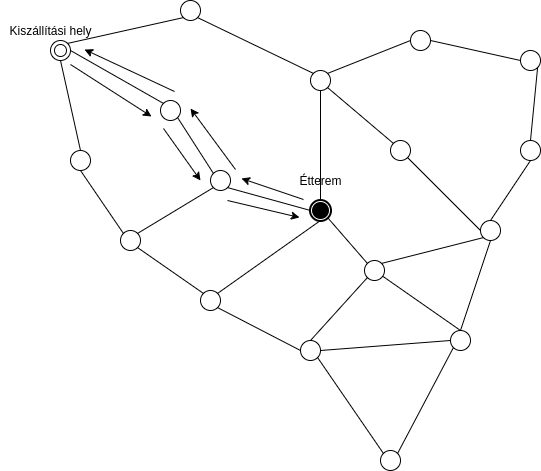
\includegraphics[scale=0.5]{images/Astar.png}
\caption{Egy étterem, egy futár, egy kiszállítás modellje}
\label{fig:model1}
\end{figure}

\Section{A probléma megoldása}

A* algoritmus

Az eljárásban a kiértékelő függvényünk a heurisztikus fügvény. Maga a fő ciklus minden iterációjánál az A*-nak meg kell határoznia az általala kiterjesztendő utat. A szakasz költségét és a célhoz érésnek költségét veszi figyelembe. Így az A* meghatározza az f(n) = g(n) + h (n) függvényt minimalizáló utat. n-nel jelölik a következő úton található csúcsot, ezáltal g(n) a kezdőpontból n-ig tartó út költsége. A heurisztikus függvényt h(n)-nel azonosítható, ez pedig nem más mint az n-től a célig vezető legolcsóbb út költését becsüli.
Az algoritmus legnagyobb hibája, hogy nem alkalmazható sok nagyméretű problémához nem praktikus, mivel a nagy memóriória igénye van, mert a meglátogatott csúcsokat eltárolja.

f(n) = g(n) + h (n) \\
g(n) - a kezdőpontból n-ig tartó út költsége \\
h(n) - n-től a célig vezető legolcsóbb út költése 

\Section{A megoldás implementálása}

Egy import-ot igényel ez pedig a cv2 ami a képek olvasására és manipulására szolgáló csomag.

\begin{python}
import cv2

\end{python}

Az osztály inicializálása a következőképpen történik. G-vel jelöljük a kezdőpontot. H-val a célt. F-el pedig a költséget.

\begin{python}
def __init__(self, parent=None, position=None):
    self.parent = parent
    self.position = position

    self.g = 0
    self.h = 0
    self.f = 0

\end{python}

A következő definiciók nélkülözhetetlenek a pontok összehasonlítási folyamatában.

\begin{python}
def __eq__(self, other):
        return self.position == other.position

def __hash__(self):
        return hash(self.position)

\end{python}

A lényegi rész maga az A* algoritmus a következő.

Létrehozunk két node-ot, a start node-ot és az end node-ot.

\begin{python}
    startNode = Node(None, start)
    startNode.g = startNode.h = startNode.f = 0
    endNode = Node(None, end)
    endNode.g = endNode.h = endNode.f = 0
\end{python}

Ezt követően inicializálunk kettő listát melyek a már látogatott pontokban adnak majd nagy segítséget (nyitott és zárt lista).

\begin{python}
    openList = []
    closedList = set()
\end{python}

Megadjuk a kezdő node-ot azáltal, hogy a nyitott listába rakjuk.

\begin{python}
    openList.append(startNode)
\end{python}

Ezt kövezően ciklust indítunk, ami addig tart amíg el nem éri a végpontot.

\begin{python}
while len(openList) > 0:
\end{python}

A cikluson belül a következőképpen határozható meg a jelenlegi node.

\begin{python}
currentNode = openList[0]
currentIndex = 0
for index, item in enumerate(openList):
       if item.f < currentNode.f:
          currentNode = item
          currentIndex = index
                
\end{python}      

A nyitott listából a zárt listába a következőképp rakjuk át az adott elemet
          
\begin{python}
openList.pop(currentIndex)
closedList.add(currentNode)
\end{python}

A célhoz vezető út meghatározása a következőképpen zajlik.

\begin{python}
if currentNode == endNode:
    path = []
    current = currentNode
    while current is not None:
        path.append(current.position)
        current = current.parent
    return path[::-1]
\end{python}

Az út meghatározásában nagy szerepet játszik a navigáció, észak, dél, kelet és nyugat irányban tudunk elindulni, köztes irányok nincsennek. Ezáltal ki van küszöbölve az a probléma, hogy ha a futár kereszteződéshez ér akkor egyből ráhajt az kívánt útra anélkül, hogy a kereszteződésbe belépne. Ehhez nekünk meg kell hatázozni a node pozicióját. Ezt kövezően egyértelművé kell hogy váljon, hogy közvetlenül el lehet-e érni. Le kell ellenőrizni, hogy az adott pont tényleg út-e. Mindezek után hozunk létre egy új node-ot amit aztán hozzáadunk az új lehetséges úthoz.

\begin{python}
newWay = []                
for newPosition in [(0, -1), (0, 1), (-1, 0), (1, 0)]:

    nodePosition = (currentNode.position[0] + newPosition[0], 
            		currentNode.position[1] + newPosition[1])

    if nodePosition[0] > (len(maze) - 1) or 
    nodePosition[0] < 0 or 
    nodePosition[1] > (len(maze[len(maze)-1]) -1) or 
    nodePosition[1] < 0:
        continue

    if maze[nodePosition[0]][nodePosition[1]] != 0:
        continue

    newNode = Node(currentNode, nodePosition)

    newWay.append(newNode)
\end{python}

Az algoritmus utolsó lépéseként pedig megvizsgáljuk ezen lehetséges utakat, kiértékeljük a már fentebb említett f, g és h értékeket majd ezek által kiválasztjuk a legkedvezőbbet.
\begin{python}
for way in newWay:

    if way in closedList:
        continue

    way.g = currentNode.g + 1
    way.h = ((way.position[0] - endNode.position[0]) ** 2) + 
    		((way.position[1] - endNode.position[1]) ** 2)
    way.f = way.g + way.h

    for openNode in openList:
        if way == openNode and way.g > openNode.g:
            continue

    openList.append(way)
\end{python}

Az implementációs rész elején említett cv2 csomag a következőkért szükséges. Adott egy kép, ami fekete(0, 0, 0), fehér(255, 255, 255), egy piros(0,0,255) és egy kék(255,0,0) színű pontokból tevődik össze. A fekete jelképezi a járhatatlan utat. Fehér színnel van jelölve a járható út. A piros szín mutatja meg a rendelési helyet, míg a kék az éttermet szimbolizálja. Ezen képfeldolgozáshoz a következők inicializálások szükségesek.

\begin{python}
img = cv2.imread("AStarProblem.bmp")
height, width, channels = img.shape

blue = "[255   0   0]"
red = "[  0   0 255]"
black = "[0 0 0]"
white = "[255 255 255]"
    
mazeHelp = []
maze = []
\end{python}

A kép minden pontján átmenve egy kettős ciklussal meghatározható a pixel pontos színe. Ebből egy tömböt kreálva elkészül az A* algoritmushoz felhasználható térkép. Futtatva az algoritmust az optimális utat kiszínezi sárga színnel az étterem és a kiszállítás helye között.

\begin{python}
for i in range(width):
    for j in range(height):
        if (str(img[i, j]) in white):
            mazeHelp.append(0)
        if (str(img[i, j]) in black):
            mazeHelp.append(1)
        if (str(img[i, j]) in red):
            mazeHelp.append(0)
            start = (i, j)
        if (str(img[i, j]) in blue):
            mazeHelp.append(0)
            end = (i, j)
    maze.append(mazeHelp)
    mazeHelp = []
path = aStar(maze, start, end)

for k in path:
    img[k] = [0, 255, 255]
cv2.imwrite('AStarResult.bmp', img)
\end{python}

\Section{A megoldás tesztelése}

A megoldás teszteléséhez nélkülözhetetlen egy bmp kép. A program megfelelő futásához elengedhetetlen, hogy a kép hosszúsága és szélessége megegyezzen. A fehér színnel kell kitelteni a járható utat, feketével a járhatatlant. Kék szín kell, hogy jelezze az éttermet, piros pedig a kiszállítási helyet. Amennyiben van lehetséges út az utóbbi két pont között, az alakalmazás megtalálja, valamint ha több út is tartozik hozzá, akkor a lehető legrövidebbet adja válaszul. Az eredmény egy képet generál, amin sárgával van feltüntetve az optimális út.

Egy kézzel rajzolt, várostérkép a következőképpen néz ki.

\begin{figure}[h!]
\centering
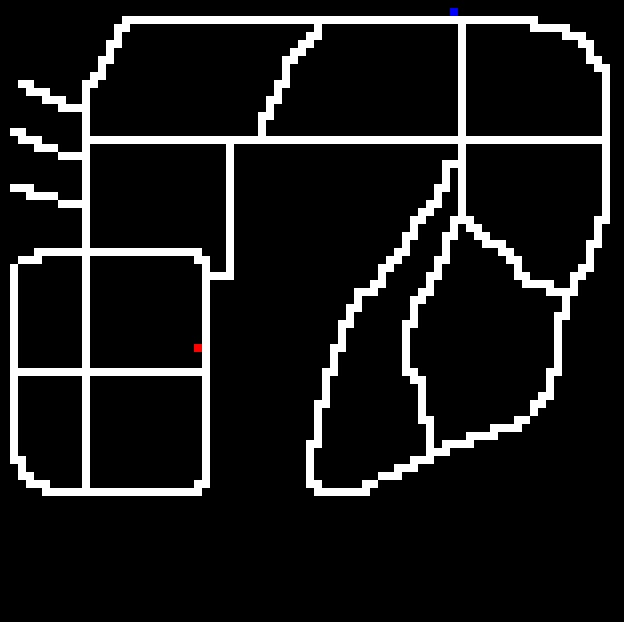
\includegraphics[scale=0.6]{images/AStarProblem.jpg}
\caption{Teszt bemenet}
\label{fig:model1problem}
\end{figure}

A megoldást felhasználva a következő képet adja válaszul.

\begin{figure}[h!]
\centering
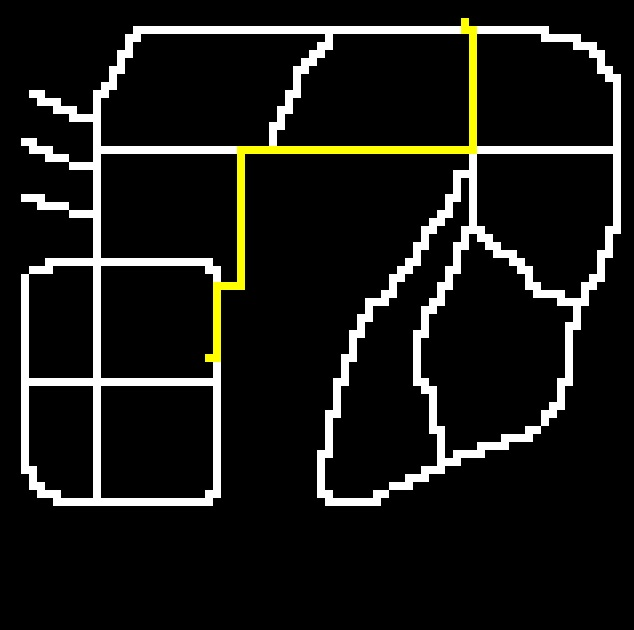
\includegraphics[scale=0.6]{images/AStarResult.jpg}
\caption{Teszt kimenet}
\label{fig:model1result}
\end{figure}

A kép kíválóan szemlélteti, hogy a optimális utat adott eredményül, ezáltal az algoritmus felhasználható az adott feladathoz.

